\documentclass[twocolumn,aps,prd,superscriptaddress]{revtex4-1}  
\usepackage{amsmath,graphicx}

\DeclareMathOperator{\Tr}{Tr}

\usepackage[usenames]{color}
\newcommand{\sv}[1]{\textcolor{blue}{\it{\textbf{sv: #1}}} }
\newcommand{\ki}[1]{\textcolor{cyan}{\it{\textbf{ki: #1}}} }

\newcommand{\Agw}{\ensuremath{A_\mathrm{gw}}}


\begin{document}

\title{Assessing spatial correlations in pulsar timing arrays with the noise-marginalized optimal statistic}


\author{Sarah J.\ Vigeland}
\affiliation{Center for Gravitation, Cosmology and Astrophysics, University of Wisconsin--Milwaukee, PO Box 413, Milwaukee WI, 53201, USA}

\author{Kristina P.\ Islo}
\affiliation{Center for Gravitation, Cosmology and Astrophysics, University of Wisconsin--Milwaukee, PO Box 413, Milwaukee WI, 53201, USA}

\author{Stephen R.\ Taylor}
\affiliation{Jet Propulsion Laboratory, California Institute of Technology, 4800 Oak Grove Drive, Pasadena, California 91106, USA}

\author{Justin A.\ Ellis}
\affiliation{Jet Propulsion Laboratory, California Institute of Technology, 4800 Oak Grove Drive, Pasadena, California 91106, USA}

\date{\today}  

\begin{abstract}
Supermassive black hole binaries (SMBHBs) are predicted to form a high-redshift cosmological population of low-frequency gravitational wave sources which added together produce a stochastic gravitational wave background (GWB) potentially measurable via pulsar timing. Comparing the actual and predicted times-of-arrival (TOAs) of radio pulses beamed by millisecond pulsars allows us to search for and place limits on the stochastic background. While most estimating of GWB significance is done via Bayesian analysis, here we use a frequentist estimator called the noise-marginalized optimal statistic to assess the significance of a GWB present in simulated PTA data. We find \ki{complete}

\end{abstract}

\maketitle


\section{Introduction}

Pulsar timing arrays (PTAs) are a conglomerate of pulsars with millisecond periods. 
Monitoring the ultra-regular periodic emission from these pulsars with radio telescopes 
enables us to probe the dynamics of the spacetime through which the pulses travel. 
PTAs are sensitive to gravitational waves (GWs) with frequencies of 
$10^{-9} - 10^{-7}\;\mathrm{Hz}$ \ki{citations needed}, 
which makes PTAs ideal complements to ground- and space-based GW detectors \sv{add citations}. 
\sv{something...} predict that the incoherent superposition of inspiraling SMBHBs form the dominant signal in this low-frequency regime \sv{add citations}.

Most measuring of the stochastic background is done through Bayesian data analysis. \ki{baye baye baye stuff} There are many advantages to running full Bayesian analyses on data sets, but they are slow. The bulk of the work consists of inverting non-diagonal matrices to find the strength of Hellings-Downs cross-correlations between pulsar pairs -- the "smoking gun" of a stochastic GWB.    

Determining the significance of various cross-correlations between pulsar pairs is computationally expensive, requiring multi-core computing clusters many days to complete. As PTA data-analysis expands to include more parameters when measuring our predicted signal, e.g. increase in residuals with continued and new pulsar observations, uncertainty in solar system ephemerides, etc., computation time will only increase. Thus methods which hasten the production of results without compromising accuracy are not only preferable, but will be necessary. Here we explore the noise-marginalized optimal statistic as an estimator for GWB signals.

The optimal statistic is a frequentist estimator for the stochastic background amplitude. 
It was derived by \citet{abc+2009} \sv{blah blah blah... try not to plagiarize myself}

The optimal statistic is an important complement to Bayesian detection techniques. 
It provides an independent way to assess the significance of the stochastic background, 
and it is significantly faster to compute. It is also easy to test different spatial correlations 
by altering the overlap reduction function (ORF) $\Gamma$ in the cross-correlations. 
In contrast, doing a full Bayesian analysis with spatial correlations is a very computationally 
intensive procedure.

However, previous work has found that the optimal statistic gives biased results \sv{expand...} 
In order to compute the optimal statistic, the timing model parameters are fixed 
at the maximum-likelihood values, but this leads to biases in the 
optimal statistic value and uncertainty due to covariances between the 
individual red noise parameters and the GW amplitude. 

In this paper, we present a technique for improving the accuracy of the optimal statistic 
by marginalizing the optimal statistic over the individual red noise parameters 
using the posterior distributions from a full Bayesian analysis. 
This hybrid approach produces a more accurate 
estimate of \Agw\ and its uncertainty.

This paper is organized as follows. In Sec.~\ref{sec:marg_os} 
we lay out the procedure for computing the noise-marginalized optimal statistic 
and compare to the fixed-noise optimal statistic. 
In Sec.~\ref{sec:spatial} determine how well 
the noise-marginalized optimal statistic can 
differentiate between different spatial correlations 
using simulated PTA data. 
In Sec.~\ref{sec:skyscrambles} we determine how well the noise-marginalized optimal statistic 
can assess the significance of a GW detection by performing sky scrambles \citep{cs2016}. 
and compare to the Bayesian analysis done by \citet{tlb+2017}. 
We conclude in Sec.~\ref{sec:conclusion}.


\section{Noise-marginalized optimal statistic}
\label{sec:marg_os}

As introduced by \citet{abc+2009}, 
the optimal statistic is derived by analytically maximizing 
the PTA likelihood function in the weak-signal regime. 
The likelihood function is given by
\begin{equation}
	p({\bf{r}}|\phi) = \frac{\exp[-\frac{1}{2} {\bf{r}}^T \Sigma^{-1}(\phi) {\bf{r}} ]}{\sqrt{\mathrm{det}[2\pi \Sigma(\phi)]}} \,,
\end{equation}
where $\bf{r}$ is an array of the timing residuals 
from the $M$ pulsars in the PTA,
\begin{equation}
	\bf{r} = \left[ \begin{array}{c} {\bf{r}}_1 \\ {\bf{r}}_2 \\ \vdots \\ {\bf{r}}_M \end{array} \right] \,,
\end{equation}
$\phi$ is the set of pulsar noise parameters, 
and $\Sigma$ is the covariance matrix of the residuals. 
We can write $\Sigma$ in terms of 
autocovariance and cross-covariance matrices ${\bf{P}}_I$ and ${\bf{S}}_{IJ}$, respectively, as
\begin{equation}
	\Sigma = \left[ \begin{array}{cccc} {\bf{P}}_1 & {\bf{S}}_{12} & \hdots & {\bf{S}}_{1M}  \\
							{\bf{S}}_{21} & {\bf{P}}_2 & \hdots & {\bf{S}}_{2M} \\
							\vdots & \vdots & \ddots & \vdots \\
							{\bf{S}}_{M1} & {\bf{S}}_{M2} & \hdots & {\bf{P}}_M \end{array} \right] \,,
\end{equation}
where
\begin{eqnarray}
	{\bf{P}} &=& \left\langle {\bf{r}}_I {\bf{r}}_I^T \right\rangle \,, \\
	{\bf{S}}_{IJ} &=& \left. \left\langle {\bf{r}}_I {\bf{r}}_J^T \right\rangle \right|_{I \neq J} \,.
\end{eqnarray}
\sv{something about the ORF...}

Analytically maximizing this likelihood gives the optimal statistic,
\begin{equation}
	\hat{A}^2 = \frac{\sum_{IJ} {\bf{r}}_I^T {\bf{P}}_I^{-1} \tilde{{\bf{S}}}_{IJ} {\bf{P}}_J^{-1} {\bf{r}}_J}{\sum_{IJ} \Tr \left( {\bf{P}}_I^{-1} \tilde{{\bf{S}}}_{IJ} {\bf{P}}_J^{-1} \tilde{{\bf{S}}}_{JI} \right) } \,,
\end{equation}
where $\tilde{{\bf{S}}}_{IJ}$ is the amplitude-independent cross-correlation matrix,
\begin{equation}
	\Agw^2 \tilde{{\bf{S}}}_{IJ} = {\bf{S}}_{IJ} \,.
\end{equation}
The normalization of $\hat{A}^2$ has been chosen so that 
$\langle \hat{A}^2 \rangle = \Agw^2$. 
For a weak GW signal, the standard deviation is 
\begin{equation}
	\sigma_0 = \left[ \sum_{IJ} \Tr \left( {\bf{P}}_I^{-1} \tilde{{\bf{S}}}_{IJ} {\bf{P}}_J^{-1} \tilde{{\bf{S}}}_{JI} \right) \right]^{-1/2} \,,
\end{equation}
and the signal-to-noise ratio (SNR) is
\begin{equation}
	\hat{\rho} = \frac{\hat{A}^2}{\sigma_0} = \frac{\sum_{IJ} {\bf{r}}_I^T {\bf{P}}_I^{-1} \tilde{{\bf{S}}}_{IJ} {\bf{P}}_J^{-1} {\bf{r}}_J}{\left[ \sum_{IJ} \Tr \left( {\bf{P}}_I^{-1} \tilde{{\bf{S}}}_{IJ} {\bf{P}}_J^{-1} \tilde{{\bf{S}}}_{JI} \right) \right]^{1/2}} \,.
\end{equation}
The expectation value of the SNR, averaged over all realizations of the stochastic background, is
\begin{equation}
	\left\langle \rho \right\rangle = \Agw^2 \left[ \sum_{IJ} \Tr\left( {\bf{P}}_I^{-1} \tilde{{\bf{S}}}_{IJ} {\bf{P}}_J^{-1} \tilde{{\bf{S}}}_{JI} \right) \right]^{1/2} \,.
\end{equation}

When constructing the optimal statistic, we typically fix the red noise parameters $\phi$ to the values that 
maximize the likelihood, which we determine from a Bayesian common red noise analysis 
\sv{check this part}. However, 
doing this biases the optimal statistic and SNR \sv{blah blah blah} 
In this paper we introduce a procedure to correct this bias by 
marginalizing over the red noise parameters using 
posterior distributions from a Bayesian analysis.

In order to compare the noise-marginalized optimal statistic to the 
fixed-noise optimal statistic, we injected a GW stochastic background with 
$\Agw = 5 \times 10^{-15}$ into simulated PTA data. 
We constructed simulated data sets using the same procedure as in \citet{tlb+2017}, 
which consisted of 10 MSPs with \sv{Steve fill in here...}

The optimal statistic was computed using the \sv{fill in...} in PAL2 \sv{add citation}. 
We incorporate the individual pulsar noise parameters as follows. 
We perform individual Bayesian noise analyses on all of the pulsars, and 
fix the white noise to the maximum likelihood value. 
To compute the fixed-noise optimal statistic, 
the red noise parameters for each pulsar are set to the mode of 
the joint posterior distribution for $A_\mathrm{red}$,$\gamma_\mathrm{red}$, 
found by performing a Bayesian common red noise analysis. 
For the noise-marginalized optimal statistic, we draw from 
the common red noise posteriors in order to average the optimal statistic over 
the individual pulsars' red noise.

Figure~\ref{fig:os_dataset_sample} shows the fixed-noise and noise-marginalized 
optimal statistic for a single realization of the stochastic background. 
We also include the distribution of $\Agw^2$ found using the results of a Bayesian analysis 
for a common red process. For this particular realization of the stochastic background, 
the values of $\hat{A}^2$ from the noise-marginalized and Bayesian analyses are in good agreement 
with each other and the injected GW stochastic background, 
but the value from the fixed-noise analysis is significantly lower. 
The noise-marginalized analysis also gives a larger mean SNR compared to the fixed-noise analysis.
\begin{figure}[ht]
	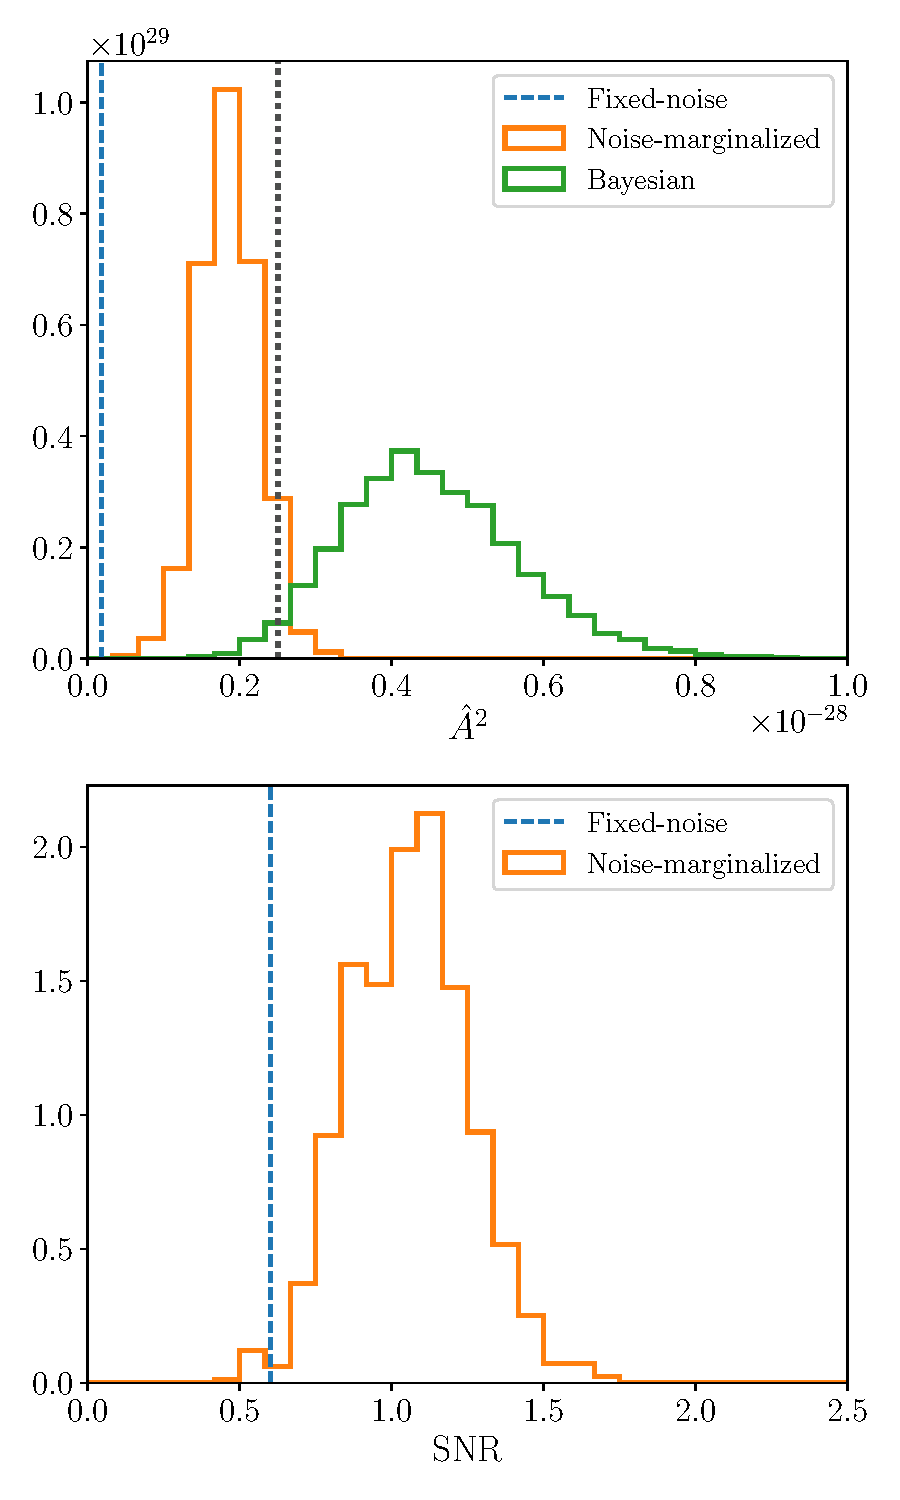
\includegraphics[width=\columnwidth]{plots/os_dataset50.pdf}
	\caption{Optimal statistic and SNR for a simulated dataset 
			containing an injected GW background with $\Agw = 5\times10^{-15}$. 
			We compare the values found using a fixed-noise analysis (dashed blue line) to the 
			mean optimal statistic and mean SNR found by marginalizing over 
			the individual pulsars' red noise parameters (solid orange line). 
			We also include the distribution of $\Agw^2$ found using the results of a Bayesian analysis 
			for a common red process (solid green line). 
			The dotted vertical line indicates the injected value, $\hat{A}^2 = 2.5 \times 10^{-29}$. 
			For this particular realization of the stochastic background, the fixed-noise analysis 
			gives $\hat{A}^2 = 1.9 \times 10^{-30}$ with $\mathrm{SNR} = 0.60$, 
			while the noise-marginalized analysis gives $\hat{A}^2 = 1.9\times10^{-29}$ with $\mathrm{SNR} = 1.1$. 
			For comparison, the Bayesian analysis gives a mean value of $\Agw^2 = 4.5\times10^{-29}$.}
	\label{fig:os_dataset_sample}
\end{figure}

Figure~\ref{fig:os_datasetstats} compares the fixed-noise values of $\hat{A}^2$ 
to the mean $\hat{A}^2$ for 425 different realizations of the stochastic background. 
The fixed-noise analysis tends to underestimate the strength of the stochastic background, 
whereas the noise-marginalized analysis is better able to recover the injected value. 
The mean value of the optimal statistic from the fixed-noise analysis, 
averaged over realizations of the stochastic background, is $\hat{A}^2 = 8.9 \times 10^{-30}$, 
while the mean value from the noise-marginalized analysis is $\hat{A}^2 = 2.5 \times 10^{-29}$. 
The noise-marginalized analysis also gives a higher average mean SNR of 1.7, 
compared to an average SNR of 1.0 using the fixed-noise analysis.
\begin{figure}[ht]
	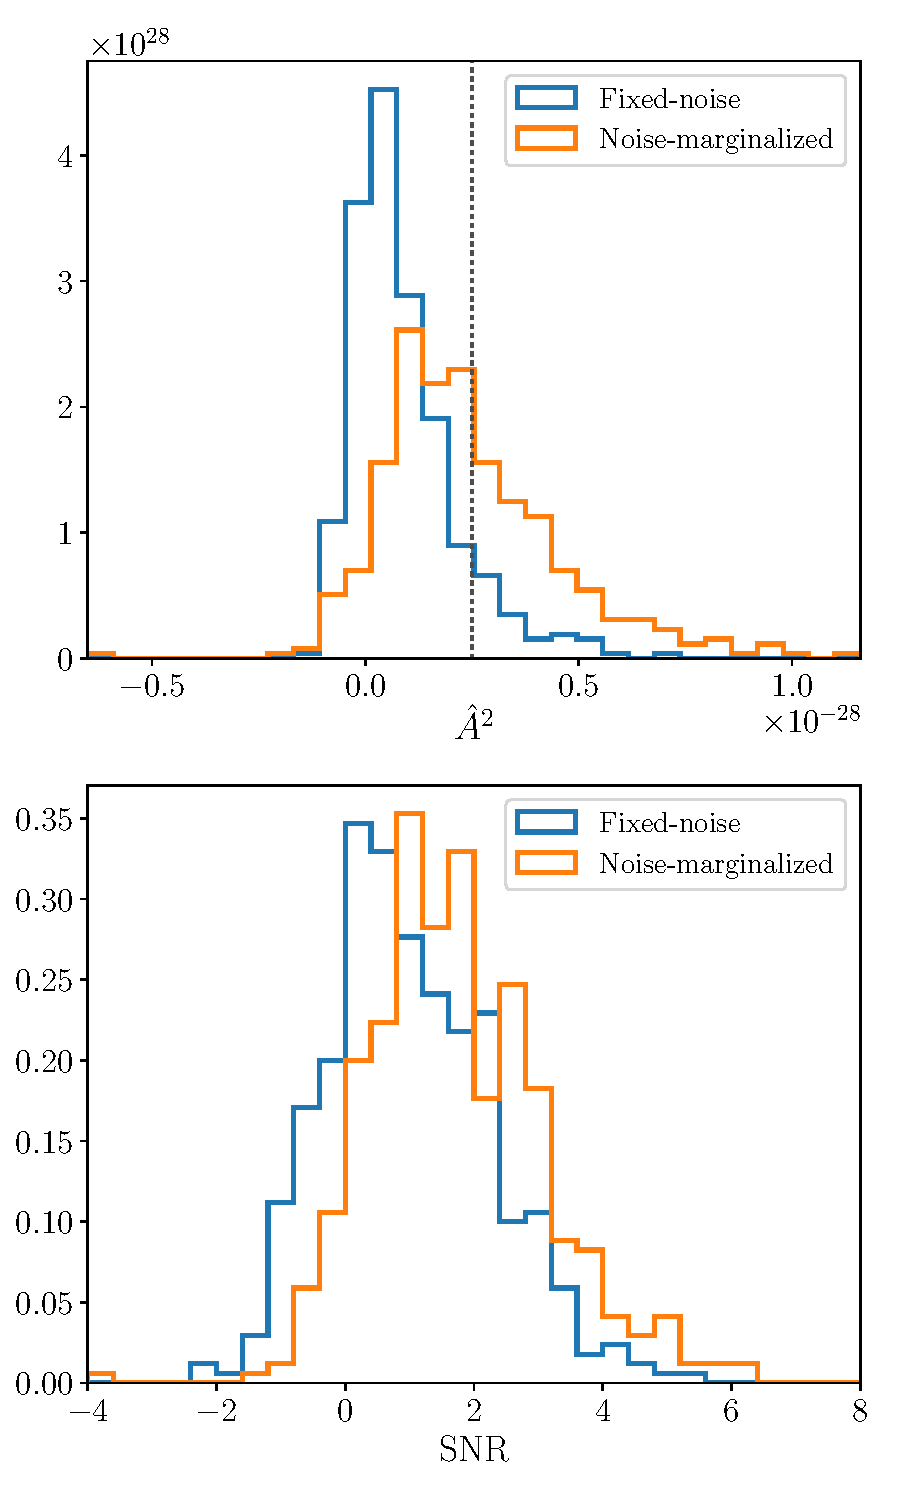
\includegraphics[width=\columnwidth]{plots/os_datasetstats_5e-15.pdf}
	\caption{Optimal statistic and SNR for 425 simulated datasets 
			containing an injected GW background with $\Agw = 5\times10^{-15}$. 
			We compare the values found using a fixed-noise analysis (blue) to the 
			mean optimal statistic and mean SNR found by marginalizing over 
			the individual pulsars' red noise parameters. The dashed vertical line 
			indicates the injected value, $\hat{A}^2 = 2.5 \times 10^{-29}$. 
			The value of $\hat{A}^2$ from the fixed-noise analysis, 
			averaged over realizations of the stochastic background, is $\hat{A}^2 = 8.9 \times 10^{-30}$, 
			while the noise-marginalized analysis gives a mean value of $\hat{A}^2 = 2.5 \times 10^{-29}$. 
			Furthermore, the fixed-noise analysis gives an average SNR of 1.0, while the 
			noise-marginalized analysis gives an average mean SNR of 1.7.}
	\label{fig:os_datasetstats}
\end{figure}


\section{Compare Significance with Monopole and Dipole}
\label{sec:spatial}

The optimal statistic is particularly well-suited to compare multiple spatial correlation relations 
because using a different spatial correlation only requires changing the ORF 
in $\tilde{{\bf{S}}}_{IJ}$. 
\citet{thk+2016} demonstrated how the optimal statistic can be altered to fit for 
multiple spatial correlations at once in order to mitigate common noise sources such as 
clock error and ephemeris error. 
Here we compute the optimal statistic with monopole and dipole spatial correlations 
for the same simulated data sets as in the previous section in order to determine 
how well we can distinguish a GW background from a monopole or dipole signal. 
For a monopole signal, the ORF becomes simply
\[ \Gamma(\theta_{IJ}) = 1 \,\]
while for a dipole signal, the ORF becomes
\[ \Gamma(\theta_{IJ}) = \cos\theta_{IJ} \,. \]

Figure~\ref{fig:os_ORF} shows the noise-marginalized mean value of $\hat{A}^2$ and the mean SNR 
computed assuming monopole, dipole, and quadrupole spatial correlations 
for 425 simulated data sets. Using a monopole or dipole ORF 
gives a lower value for the mean optimal statistic and mean SNR compared to the 
Hellings-Downs ORF. 
However, there is significant overlap between the distributions for the mean SNR using 
monopole, dipole, and quadrupole ORFs, indicating that it is not easy to differentiate 
between those three spatial correlations for an injected GW background of this amplitude. 
We find a noise-marginalized mean SNR above 1.0 in 68\% of our simulated data sets 
using the quadrupole ORF, and in 45\% and 24\% of our simulated data sets 
using the monopole and dipole ORF, respectively.
\begin{figure}[ht]
	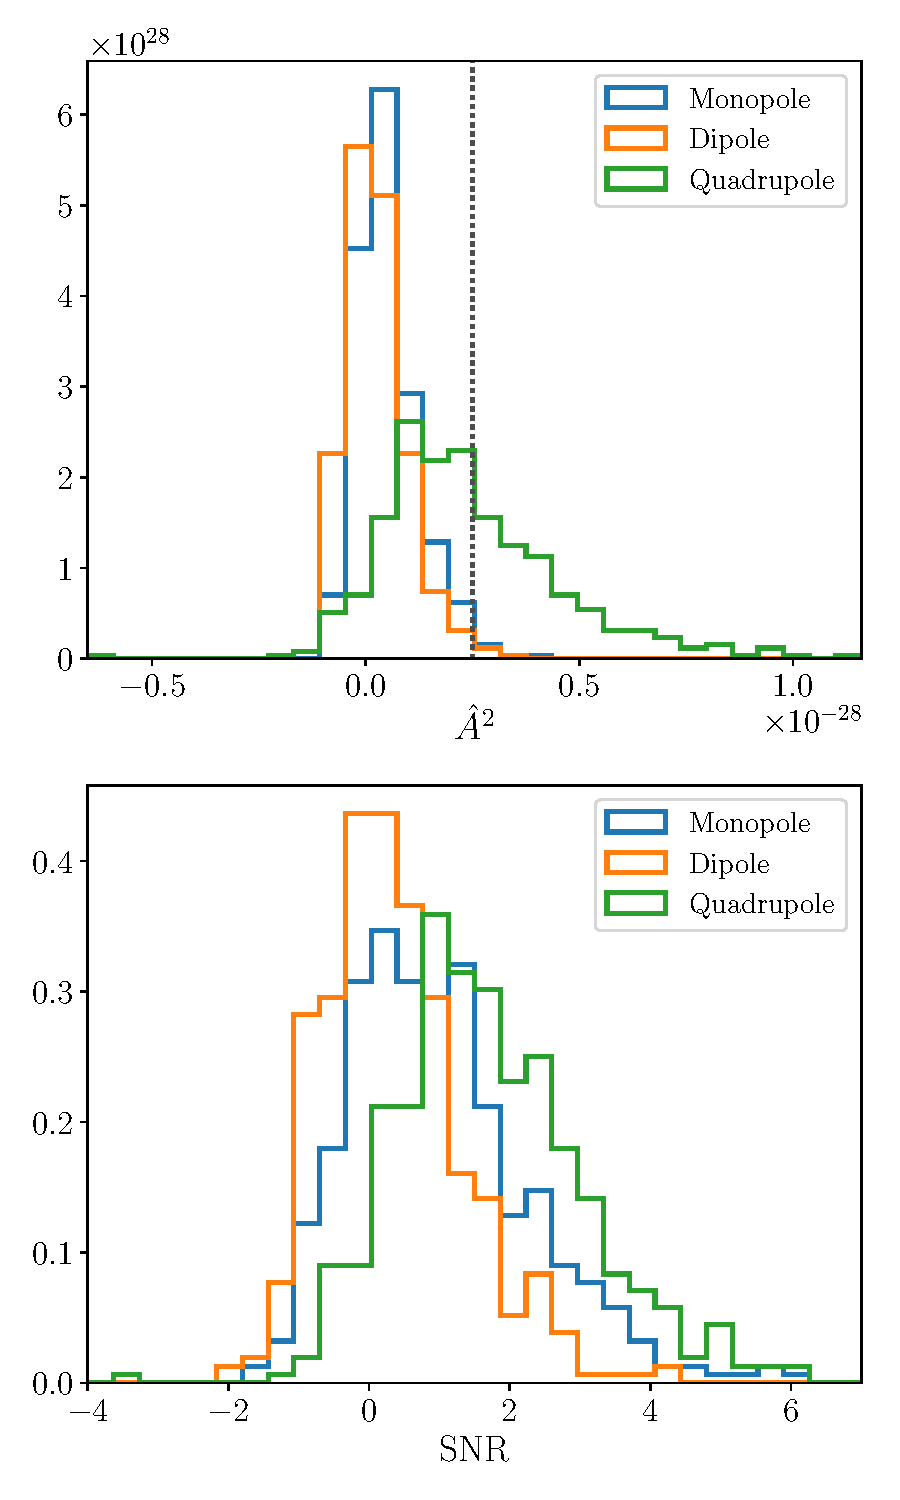
\includegraphics[width=\columnwidth]{plots/os_datasetstats_5e-15_ORF.pdf}
	\caption{Noise-marginalized mean optimal statistic and mean SNR for 425 simulated datasets 
			containing an injected GW background with $\Agw = 5\times10^{-15}$. 
			We compare the values found using monopole (blue), dipole (orange), and quadrupole (green) 
			spatial correlations. 
			The dashed vertical line indicates the injected value, $\hat{A}^2 = 2.5 \times 10^{-29}$.}
	\label{fig:os_ORF}
\end{figure}


\section{Compare Significance with Sky Scrambles/Phase Shifts}
\label{sec:skyscrambles}

Another technique for testing the spatial correlations is through ``sky scrambles,'' 
where the ORF is altered in order to simulate changing the pulsars' positions \citep{cs2016}. 
\citet{tlb+2017} showed how sky scrambles affect the Bayes' factor for simulated data sets. 
Here we perform a similar analysis using frequentist methods.

The scrambled sky positions were generated \sv{Steve, explain here...}

Figure~\ref{fig:skyscrambles_dataset_sample} compares the noise-marginalized optimal statistic 
for a particular data set to the 
distribution of noise-marginalized optimal statistics obtained using sky scrambles.
\sv{sky scrambles for all of our simulated data sets}

\begin{figure}[ht]
	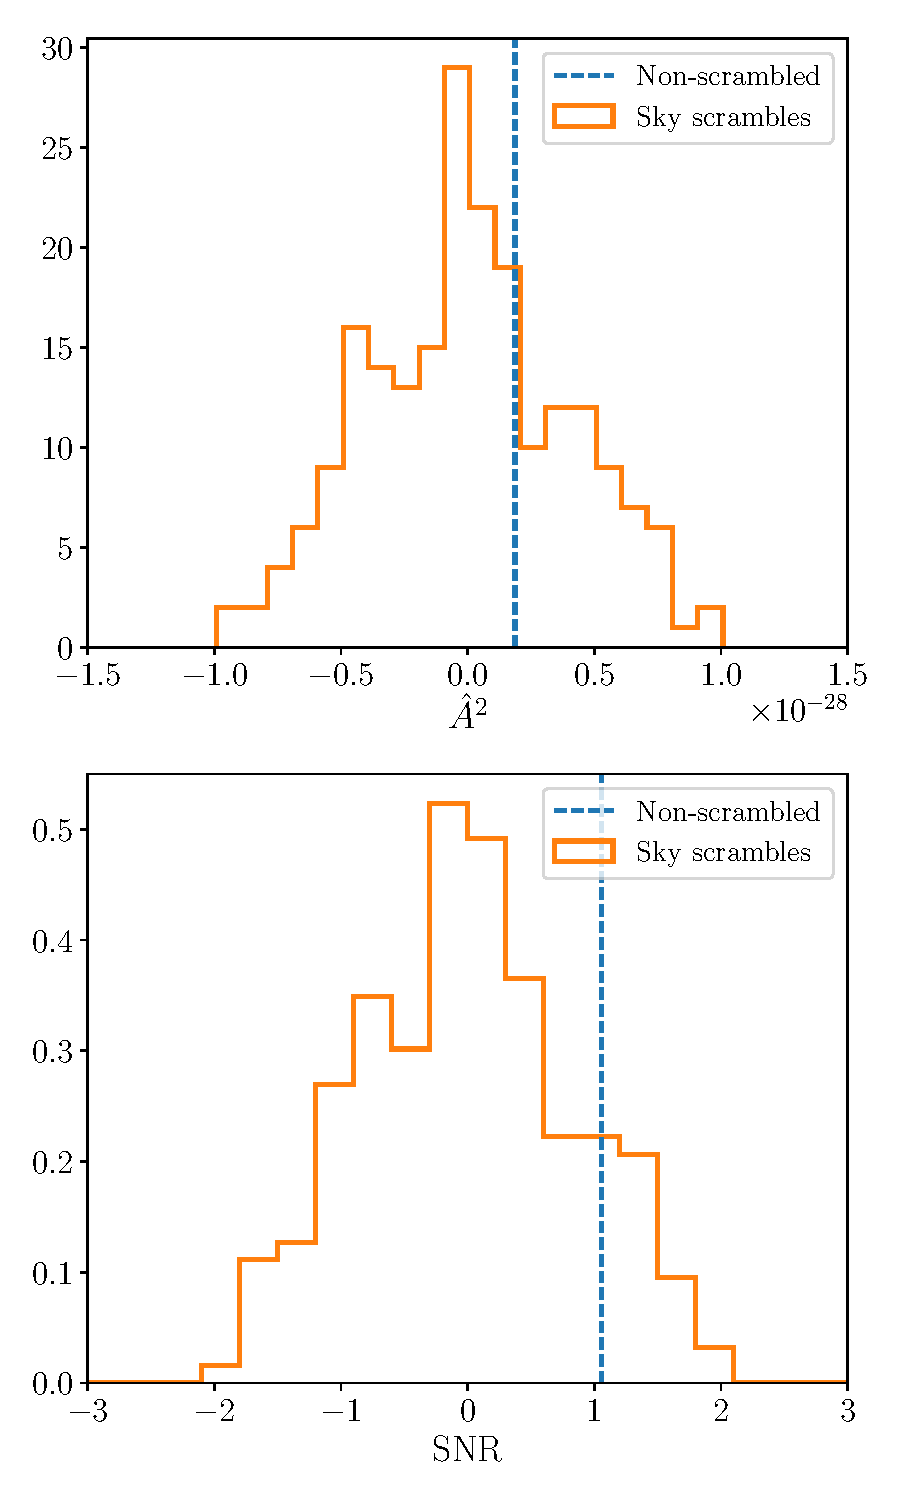
\includegraphics[width=\columnwidth]{plots/skyscrambles_dataset50.pdf}
	\caption{Comparison between the optimal statistic with and without sky scrambles 
			for a simulated dataset containing an injected GW background with $\Agw = 5\times10^{-15}$. 
			The true analysis found an $\mathrm{SNR} = 1.1$, while only 24 of the 210 sky scramble analyses 
			found $\mathrm{SNR} \geq 1.1$ ($p=0.11$).}
	\label{fig:skyscrambles_dataset_sample}
\end{figure}

\sv{comparison to Steve's}


\section{Conclusion}
\label{sec:conclusion}


\acknowledgments
We thank Joe Romano and Xavier Siemens for useful discussions. 
JAE was supported by NASA through Einstein Fellowship Grant PF4-150120. 
SRT was supported by appointment to the NASA Postdoctoral Program 
at the Jet Propulsion Laboratory, which is administered by Oak Ridge Associated Universities 
and the Universities Space Research Association through a contract with NASA. 
KPI and SJV are supported by NSF Physics Frontier Center Grant 1430284.


\bibliographystyle{apsrev}
\bibliography{master}

\end{document}